% =============================================================================
% Section: Do fine-tuned models reason in superposition?
% Standalone section — Coconut (Hao et al., 2024) reproduction & analysis
% =============================================================================

\section{Do Fine-Tuned Models Reason in Superposition?}
\label{sec:coconut}

% ---------------------------------------------------------------------------
% 5.1  Background & Setup
% ---------------------------------------------------------------------------
\subsection{Background}
\label{sec:coconut-background}

\begin{itemize}
    \item Coconut~\cite{hao2024coconut} replaces discrete chain-of-thought (CoT) tokens with \emph{continuous latent thoughts}: the model's last hidden state is fed back as the next input embedding, enabling ``reasoning in continuous latent space.''
    \item The authors claim latent tokens encode a breadth-first search (BFS) over ProsQA graphs, citing logit-lens probing that shows intermediate entities appearing at latent positions.
    \item We reproduce their ProsQA experiments (GPT-2, 5-hop graph traversal) and apply more rigorous probing to test whether latent tokens contribute meaningfully to inference.
\end{itemize}

% ---------------------------------------------------------------------------
% 5.2  Experimental Setup
% ---------------------------------------------------------------------------
\subsection{Experimental Setup}
\label{sec:coconut-setup}

\begin{itemize}
    \item \textbf{Models}: GPT-2 (124M) fine-tuned on ProsQA, a synthetic graph-traversal QA task.
    \item \textbf{CoT baseline}: Standard chain-of-thought supervised fine-tuning (85.3\% val accuracy, checkpoint epoch 49).
    \item \textbf{Coconut model}: Staged curriculum that progressively replaces CoT steps with latent tokens (99\% val accuracy, checkpoint epoch 50). Uses 6 latent tokens at full stage.
    \item \textbf{Probing methodology}: We project hidden states at each reasoning position through the LM head to obtain $P(\text{entity})$ distributions over all graph entities, then normalize across entities.
\end{itemize}

\paragraph{Methodological correction.}
\begin{itemize}
    \item The original paper probes latent positions using the \emph{final} hidden states (after all forward passes are complete). We call this the \texttt{final\_state} method.
    \item This is misleading: at position $k$, the hidden state has already been influenced by all subsequent latent passes via the accumulated KV cache. It is analogous to probing CoT step 1 after the model has already seen steps 2--5.
    \item We instead use \texttt{per\_pass} probing: at latent step $k$, we probe the hidden state immediately after the $k$-th forward pass, before any subsequent passes occur. This gives a fair comparison with CoT, where each step's probe reflects only the reasoning completed up to that point.
\end{itemize}

% ---------------------------------------------------------------------------
% 5.3  Ablation: Latent tokens are unnecessary
% ---------------------------------------------------------------------------
\subsection{Latent Tokens Are Unnecessary}
\label{sec:coconut-nolatent}

\begin{itemize}
    \item \textbf{Smoking gun}: We evaluate the trained Coconut model by feeding \emph{only the question} — no latent tokens, no multi-pass recurrence — and greedily decoding the answer.
    \item Result: the model achieves \textbf{96.6\% accuracy} (483/500) without any latent reasoning (Table~\ref{tab:coconut-accuracy}).
    \item This means the latent tokens are decorative: the model has learned to extract the answer directly from the question embedding.
\end{itemize}

\begin{table}[h]
\centering
\caption{ProsQA accuracy under different reasoning conditions.}
\label{tab:coconut-accuracy}
\begin{tabular}{lcc}
\toprule
\textbf{Condition} & \textbf{Accuracy} & \textbf{Correct / Total} \\
\midrule
CoT (discrete, 5-hop)          & 85.3\% & --- \\
Coconut (6 latent tokens)      & 99.0\% & --- \\
Coconut (no latent tokens)     & 96.6\% & 483 / 500 \\
\bottomrule
\end{tabular}
\end{table}

% ---------------------------------------------------------------------------
% 5.4  Prior belief: answer known before reasoning
% ---------------------------------------------------------------------------
\subsection{The Answer Is Known Before Reasoning Begins}
\label{sec:coconut-prior}

\begin{itemize}
    \item We probe the model's belief about the target entity \emph{immediately after processing the question}, before any latent tokens or CoT steps are generated.
    \item \textbf{Coconut}: Mean normalized $P(\text{target}) = 0.82$ at step 0, with 87\% of examples already exceeding $P(\text{target}) > 0.5$ before any reasoning.
    \item \textbf{CoT}: $P(\text{target}) \approx 0$ before reasoning — the model genuinely does not know the answer yet and must reason through intermediate steps.
    \item This asymmetry is shown in Figure~\ref{fig:question-only}: the Coconut model's prior belief is dominated by the target entity across all graph complexities, while the CoT model assigns negligible probability to the target before reasoning.
\end{itemize}

\begin{figure}[t]
    \centering
    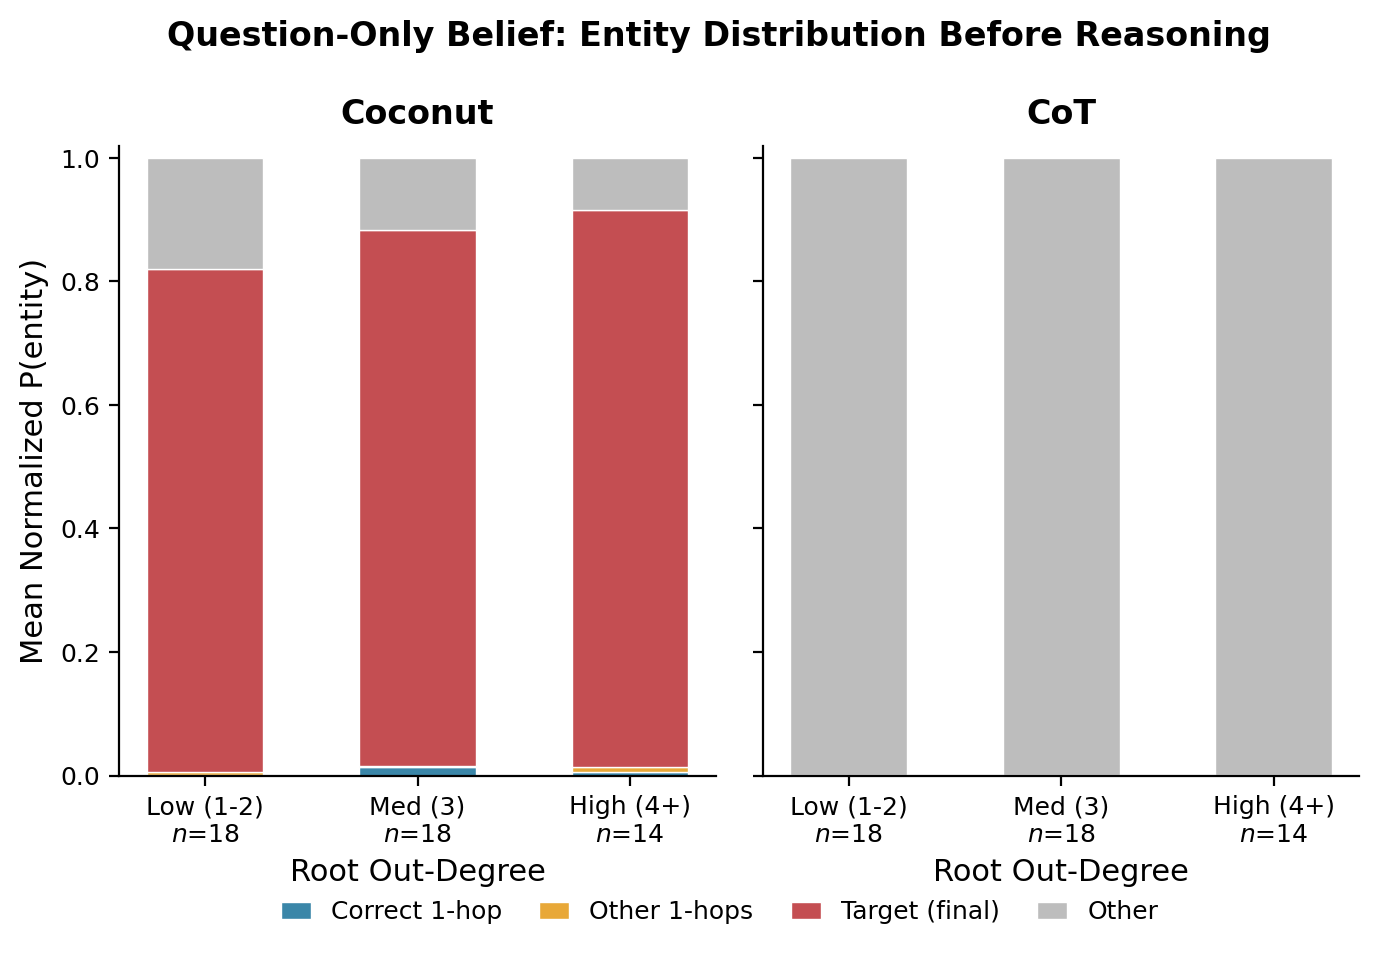
\includegraphics[width=\linewidth]{figures/question_only_belief.png}
    \caption{Entity distribution \emph{before any reasoning}. Coconut (left) already assigns $\sim$82\% normalized probability to the target. CoT (right) has near-zero target probability, with mass spread across non-target entities.}
    \label{fig:question-only}
\end{figure}

% ---------------------------------------------------------------------------
% 5.5  Belief evolution: flat vs. progressive
% ---------------------------------------------------------------------------
\subsection{Belief Does Not Evolve During Latent Reasoning}
\label{sec:coconut-evolution}

\begin{itemize}
    \item Using \texttt{per\_pass} probing, we track how the normalized entity distribution changes across reasoning steps. At each step $k$, we categorize all graph entities into four groups: \emph{correct next} (the entity the model should traverse to at step $k$), \emph{wrong neighbors} (other outgoing neighbors of the current node), \emph{target} (the final answer entity), and \emph{other}. We normalize probabilities across all entities and plot as stacked areas summing to 1 (Figure~\ref{fig:belief-evolution}).
    \item \textbf{Coconut}: The target (red) dominates from step 0 onward, occupying $>$80\% of the normalized probability mass at every latent step. The correct-next entity (blue) never surfaces as the dominant category. The distribution is essentially flat — latent computation does not shift belief.
    \item \textbf{CoT}: The correct-next entity (blue) dominates early steps, reflecting that the model is actively tracking the current intermediate in the graph traversal. At the final step, the target (red) takes over as the correct-next entity \emph{is} the target. This is the expected signature of step-by-step multi-hop reasoning.
    \item This pattern holds across both 4-step and 5-step examples (Figure~\ref{fig:belief-evolution-4step},~\ref{fig:belief-evolution-5step}), ruling out graph-depth as a confound.
\end{itemize}

\begin{figure}[t]
    \centering
    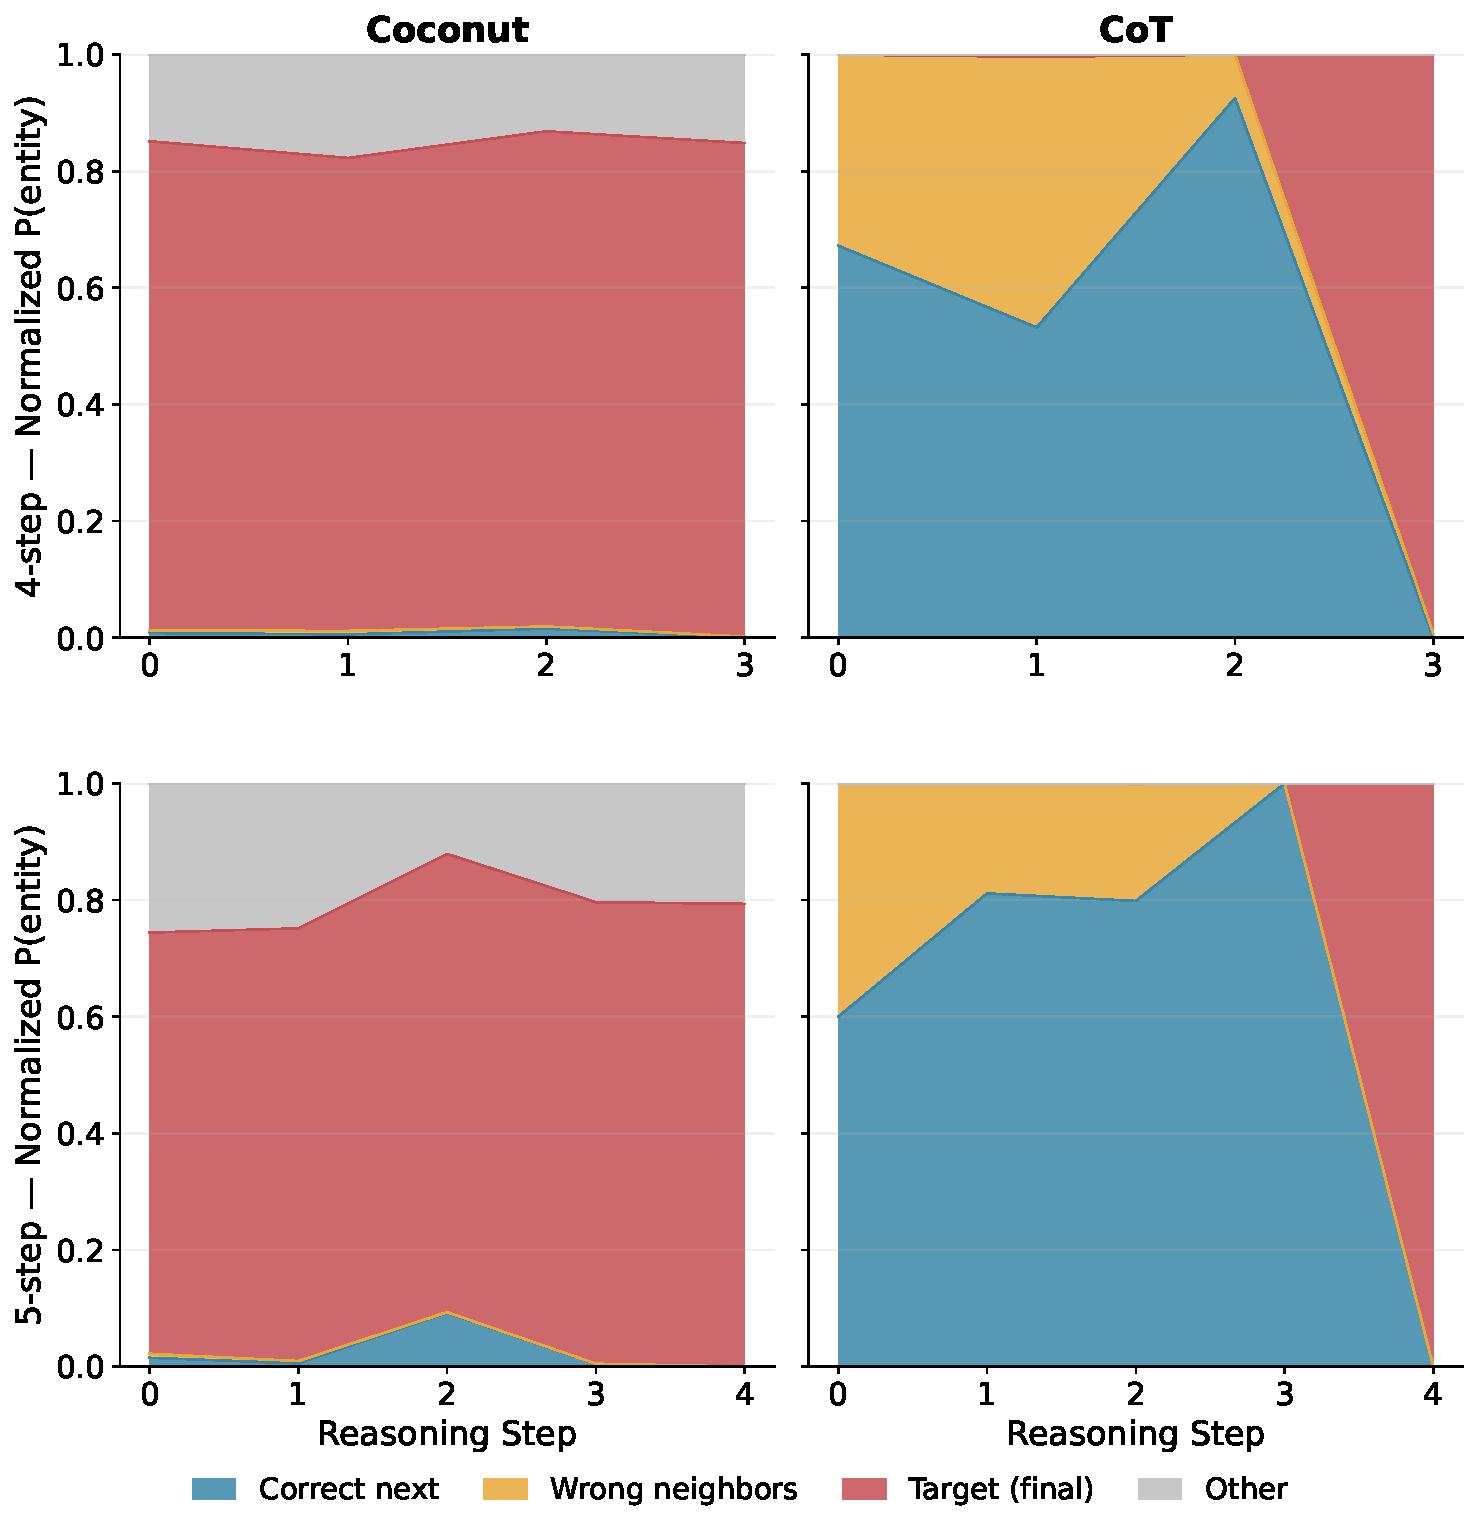
\includegraphics[width=\linewidth]{figures/stepwise_grid.pdf}
    \caption{Step-aware entity belief (normalized among all entities). \textbf{Left column (Coconut)}: target entity (red) dominates from step 0 onward with no progression. \textbf{Right column (CoT)}: correct-next entity (blue) dominates early steps, target (red) takes over at the final step. Pattern holds across 4-step (top) and 5-step (bottom) examples.}
    \label{fig:belief-evolution}
\end{figure}

% ---------------------------------------------------------------------------
% 5.6  Individual examples
% ---------------------------------------------------------------------------
\subsection{Case Study: Latent vs.\ Discrete Reasoning Traces}
\label{sec:coconut-examples}

\begin{itemize}
    \item Figure~\ref{fig:example-trace} shows a representative 4-hop example (Sally $\to$ zhorpus $\to$ zumpus $\to$ vumpus $\to$ worpus).
    \item \textbf{Coconut}: The target entity (\texttt{worpus}) dominates from T1 onward ($>$90\% normalized probability). No intermediate entities ever surface.
    \item \textbf{CoT}: Step S1 places mass on the 1-hop intermediate (\texttt{zhorpus}), S2--S3 shift through later intermediates, and S4 converges on the target. This is the expected signature of sequential graph traversal.
\end{itemize}

\begin{figure}[t]
    \centering
    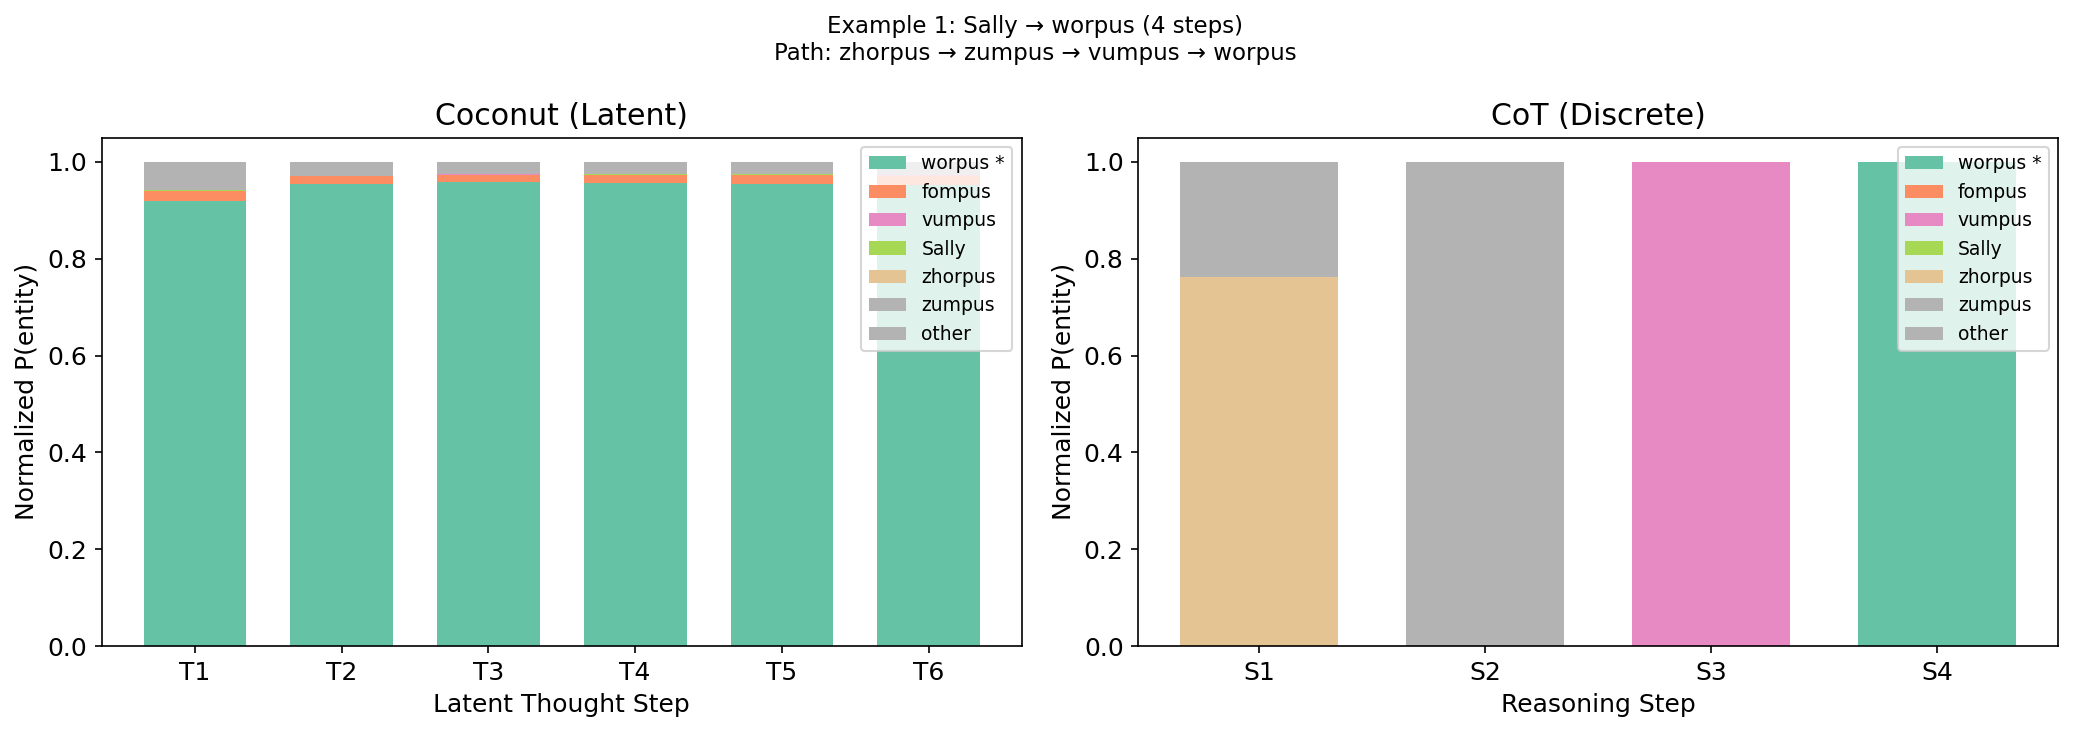
\includegraphics[width=\linewidth]{figures/bars_example_1.png}
    \caption{Per-step entity distribution for a 4-hop example. Coconut (left) locks onto the final target immediately. CoT (right) traverses intermediate entities step by step.}
    \label{fig:example-trace}
\end{figure}

% ---------------------------------------------------------------------------
% 5.7  Entropy analysis
% ---------------------------------------------------------------------------
\subsection{Entropy Confirms Absence of Deliberation}
\label{sec:coconut-entropy}

\begin{itemize}
    \item We compute the Shannon entropy of the normalized entity distribution at each reasoning step (restricted to 4-step examples for controlled comparison).
    \item \textbf{Coconut}: Entropy is approximately constant ($\sim$0.3 bits) across all 6 latent steps, indicating the model maintains a fixed, low-uncertainty belief throughout.
    \item \textbf{CoT}: Entropy rises at step 2 (peak uncertainty when multiple paths are possible) then decreases monotonically to $\sim$0.03 bits by step 4 — the expected signature of progressive disambiguation.
    \item The flat Coconut entropy is consistent with a model that has already ``decided'' and is not performing meaningful computation during latent steps (Figure~\ref{fig:entropy}).
\end{itemize}

\begin{figure}[t]
    \centering
    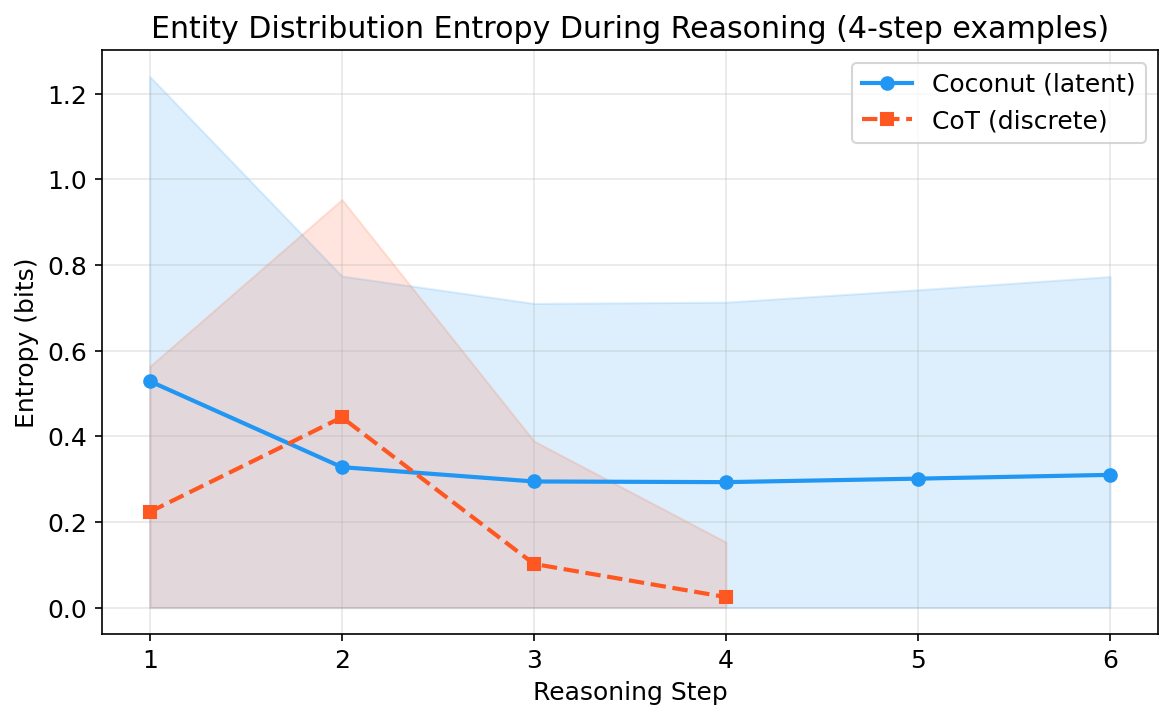
\includegraphics[width=0.75\linewidth]{figures/entropy_4step.png}
    \caption{Entity distribution entropy during reasoning (4-step examples). CoT (orange) shows the expected rise-then-fall pattern of progressive reasoning. Coconut (blue) remains flat, consistent with no deliberation.}
    \label{fig:entropy}
\end{figure}

% ---------------------------------------------------------------------------
% 5.8  Discussion
% ---------------------------------------------------------------------------
\subsection{Discussion}
\label{sec:coconut-discussion}

\begin{itemize}
    \item All evidence converges: the Coconut model solves ProsQA by learning to extract the answer from the question embedding alone, not by performing multi-hop reasoning in latent space.
    \item The original paper's probing methodology (\texttt{final\_state}) inflates the appearance of intermediate reasoning by allowing later passes to retroactively influence earlier representations via the KV cache.
    \item The 96.6\% no-latent accuracy, the 0.82 prior $P(\text{target})$, and the flat belief evolution collectively demonstrate that latent tokens are not load-bearing.
    \item \textbf{Caveat}: This does not prove that continuous latent reasoning \emph{cannot} work — only that the Coconut training procedure on ProsQA does not produce it. The model finds a shortcut (memorizing question$\to$answer mappings) rather than learning the intended multi-hop algorithm.
    \item This result motivates the question: under what conditions, if any, do latent reasoning tokens carry genuine computational content? We address this in Sections~\ref{sec:TODO} and~\ref{sec:TODO}.
\end{itemize}

% ---------------------------------------------------------------------------
% Appendix: Logit Lens
% ---------------------------------------------------------------------------
\subsection{Logit Lens Analysis}
\label{sec:coconut-logitlens}

\begin{itemize}
    \item As a complementary analysis, we apply logit lens~\cite{nostalgebraist2020logitlens} to both models: at each thinking position (latent tokens for Coconut, step-end tokens for CoT), we extract the hidden state at every transformer layer $\ell \in \{0, \ldots, 11\}$, project it through the final layer norm and LM head, and compute the Shannon entropy of the resulting vocabulary distribution.
    \item Each point in Figure~\ref{fig:logitlens} shows the average entropy at layer $\ell$, where the average is taken first across all thinking positions within an example, then across all examples ($n = 300$). Shaded regions show $\pm 1$ standard deviation across examples.
    \item \textbf{CoT}: High entropy in early/middle layers ($\sim$4 nats at layer 1--6), dropping sharply to near zero by layers 8--9. This indicates gradual refinement — early layers maintain broad uncertainty, and the model progressively commits to specific tokens in later layers.
    \item \textbf{Coconut}: Entropy is uniformly low across all layers ($<$1.5 nats), indicating that the model's hidden states at latent positions are already near-deterministic even at early layers. The representations carry little information content that would suggest active computation.
    \item The late-layer spike in CoT entropy (layers 10--11) likely reflects the model broadening over surface-form variations of the committed entity (e.g., capitalization, spacing).
\end{itemize}

\begin{figure}[t]
    \centering
    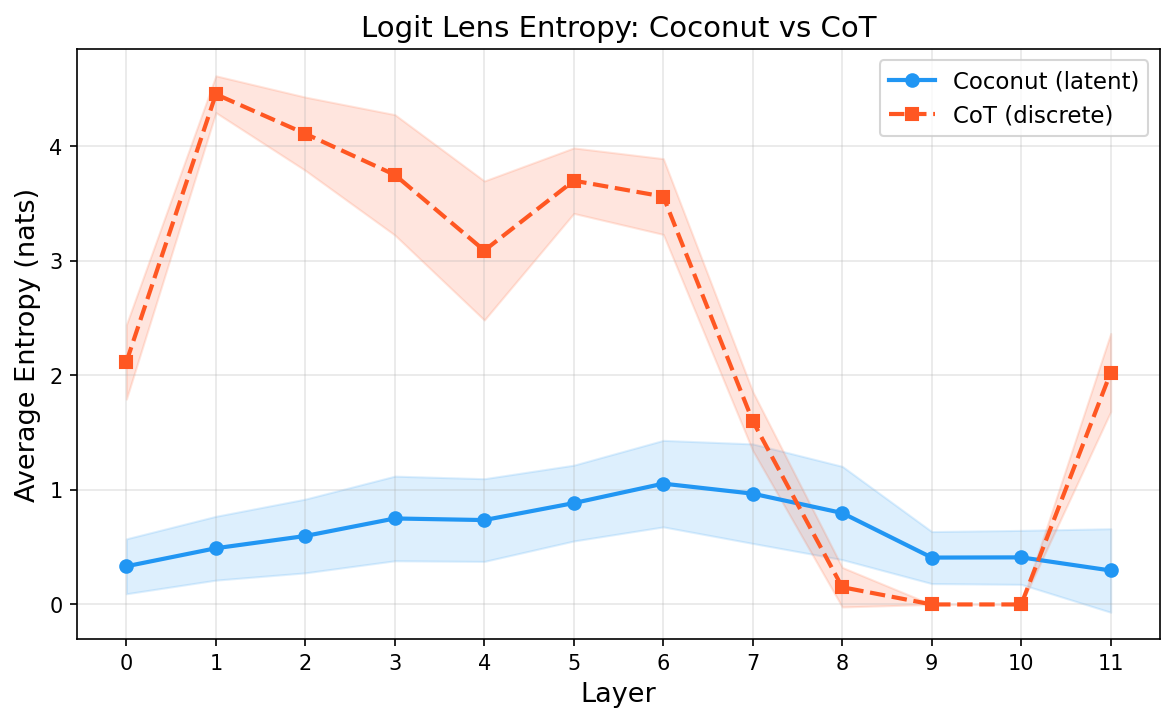
\includegraphics[width=0.75\linewidth]{figures/entropy_comparison_prosqa.png}
    \caption{Logit lens entropy across transformer layers at thinking positions. Each point: mean entropy at layer $\ell$, averaged first over positions within each example, then over all examples ($\pm 1$ std). CoT shows high early-layer entropy that resolves by layer 8--9. Coconut maintains uniformly low entropy, consistent with latent positions carrying minimal information.}
    \label{fig:logitlens}
\end{figure}
